\subsubsection{Low-Pass Filter}\label{sect:low-pass}

The low-pass filter has been realized on top of the FFT Filter,
by setting up frequency response to zero for frequencies
past certain threshold chosen heuristically
based on the window size where to cut off. We filtered out
all the frequencies past 2853 Hz.

Figure \ref{fig:low-pass} presents FFT of a
low-pass filtered graph.

\begin{figure}
	\centering
	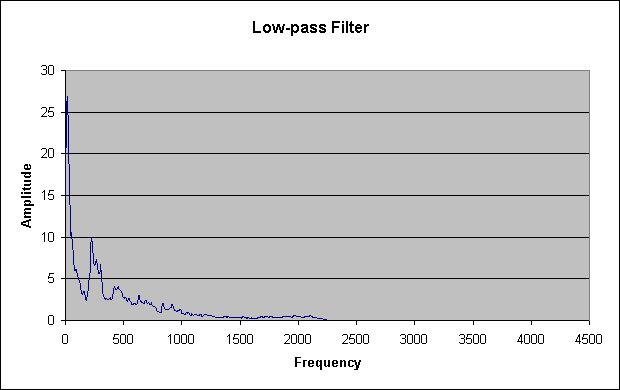
\includegraphics[width=400pt]{../graphics/graphs/low-pass-filter.png}
	\caption{Low-pass filter applied to aihua5.wav.}
	\label{fig:low-pass}
\end{figure}
